\chapter{Preliminaries}
\label{cap:prelim}

The objective of this chapter is to provide a comprehensive overview that
defines the scope of the thesis. It covers essential theoretical and technical
concepts necessary to comprehend the experiments and the architecture proposed
in subsequent chapters.

\section{Artificial Intelligence}

\textit{AI} is one of the newest fields in science and engineering. Work
started in earnest soon after World War II, and the name itself was coined in
1956 attributed by John McCarthy of MIT. \\

After successfully decrypting Enigma\footnote{Enigma was a rotor machine
designed to encrypt and decrypt messages.}, in World War II, the mathematician
Alan Turing posed a groundbreaking question that had a profound impact on
society: "Can machines think?" \cite{CanMachineThink}. In this seminal work,
Turing not only outlined the process of developing intelligent machines but
also presented a method for assessing their intelligence. Even today, the
Turing Test remains a widely recognized benchmark for evaluating the
intelligence of artificial systems. According to this test, if a human cannot
distinguish, through a text-based conversation, whether they are interacting
with a human or a machine, the artificial system can be considered to possess
intelligence. \\

The term "AI" is exciting but, the definition of this term is blurry
\cite{AIModernApprouch}. Historically there are two approaches to \textit{AI}
that have been followed, each by different people with different methods. The
human-centered approach and the rationalist approach. The incorporation of a
human-centered approach into the field must incorporate empirical scientific
methods, which entail making observations and formulating hypotheses about
human behavior. On the other hand, a rationalist approach combines the
disciplines of mathematics and engineering. These different perspectives have
both faced criticism and received praises. \\

From that juncture until the turn of the century, the field of \textit{AI}
encountered fluctuations, witnessing periods of remarkable accomplishments
interspersed with the infamous \textit{AI} winters. Currently \textit{AI} is a
hot topic of discussion, evident from the increasing searches and online
mentions. While \textit{AI} has been around for more than 65 years, the recent
exponential trend can be attributed to the availability of cost-efficient
storage, transfer, and computation capabilities for massive amounts of data.
This newfound capacity was previously unimaginable and has contributed to the
current \textit{AI} boom. \\

\textit{AI} has expanded into numerous distinct fields, showcasing its
extensive range of applications, techniques, and interdisciplinary nature. The
diversity of branches in the field of artificial intelligence is represented in
Figure \ref{fig:ai_branches}, which depicts several current
\textit{AI} fields. However, it is important to note that the figure can be
further expanded to include additional fields, such as Speech Processing and
Expert Systems, among others.

\begin{figure}[H]
  \centering
  \resizebox{0.8\textwidth}{!}{%
    \begin{tikzpicture}[mindmap, grow cyclic, every node/.style=concept, concept color=black!70, text = white,
      level 1/.append style={level distance=4.5cm,sibling angle=60},
      level 2/.append style={level distance=3cm,sibling angle=40},
      level 3/.append style={level distance=2cm,sibling angle=40}]

      \node{AI}
      child [concept color=blue!40, text = black] { node {Machine Learning}
      child [concept color=blue!25]{ node {Superv. Learning}}
      child [concept color=blue!25]{ node {Unsuperv. Learning}
      child [concept color=blue!15]{ node {Clustering}}
      child [concept color=blue!15]{ node {Pattern mining}}
      }
      child [concept color=blue!25]{ node {Reinf. Learning}}
      }
      child [concept color=orange!50, text = black] { node {Natural language processing}
      child { node {Automatic Translation}}
      child { node {Sentiment Analysis}}
      child { node {Text generation}}
      child { node {Chatbots}}
      }
      child [concept color=lime!50, text = black] { node {Optimization}
      child [concept color=lime!30]{ node {Particle Swarm Optim.}}
      child [concept color=lime!30]{ node {Evolutionary Algorithms}}
      child [concept color=lime!30]{ node {Genetic Algorithms}}
      }
      child [concept color=teal!50, text = black] { node {Robotics}
      child [concept color=teal!35]{ node {Aerial robotics}}
      child [concept color=teal!35]{ node {Manipulation}}
      child [concept color=teal!35]{ node {Locomotion}}
      child [concept color=teal!35]{ node {Multi-robot systems}
      child [concept color=teal!15]{ node {Swarm robotics}}
      child [concept color=teal!15]{ node {Formation control}}
      }
      child [concept color=teal!35]{ node {Sensing}}
      }
      child [concept color=red!50, text = black] { node {Vision}
      child [concept color=red!30]{ node {Motion analysis}}
      child [concept color=red!30]{ node {Image/scene reconstruction}}
      child [concept color=red!30]{ node {Recognition}
      child [concept color=red!15]{ node {Object recog.}}
      child [concept color=red!15]{ node {Facial recog.}}
      }
      }
      child [concept color=amber!30, text = black] { node {Planning \& Scheduling}
      child { node {SAT / MAXSAT}}
      child { node {Probabilistic planning}}
      child { node {Temporal planning}}
      };
    \end{tikzpicture}%
    }
    \caption[AI Sub-Specialists]{\textit{AI Sub-Specialists. Note that these subfields often intersect and combine. }}
    {\label{fig:ai_branches}}
\end{figure}

\newpage

\section{Machine Learning}

Machine learning (ML) is a branch of artificial intelligence (\textit{AI}) and
computer science which focuses on the use of data and algorithms to imitate the
way that humans learn, gradually improving its accuracy
\cite{IBMMachineLearning}. \\

The central idea of machine learning is the existence of a mathematical
relationship between any combination of input and output data. Rather than
manually programming knowledge into computers, machine learning endeavors to
automatically learn significant relationships and patterns by observing
examples. \\

There are three subcategories (Figure \ref{fig:ml_branches}) of
machine learning \cite{MITML}.

\begin{itemize}
  \item \textbf{Supervised Learning}

    Machine learning models are trained with labeled data sets, which allow
    the models to learn and grow more accurate over time. For example, an
    algorithm would be trained with pictures of dogs and other things, all
    labeled by humans, and the machine would learn ways to identify pictures
    of dogs on its own. Supervised machine learning is the most common type
    used today.

  \item \textbf{Unsupervised Learning}

    Unsupervised learning involves using a training set that comprises
    unlabeled inputs, meaning inputs that do not have any assigned desired
    output. The primary objective of this learning approach is to uncover
    concealed patterns or data clusters without relying on human
    intervention.

  \item \textbf{Reinforcement Learning}

    Reinforcement learning occupies a position between supervised and
    unsupervised learning. In a certain sense, there is some form of
    supervision, but it does not involve explicitly specifying a desired
    output for every input in the data. Instead, a reinforcement learning
    algorithm receives feedback from the environment only after selecting an
    output, known as an action, based on a given input or observation. The
    feedback indicates the extent to which the action fulfills the learner's
    goals.

\end{itemize}

\newpage

\begin{figure}[H]
  \centering
  \resizebox{0.6\textwidth}{!}{%
    \begin{tikzpicture}[mindmap, grow cyclic, every node/.style=concept, concept color=blue!40, text = black,
      level 1/.append style={level distance=4.5cm,sibling angle=120},
      level 2/.append style={level distance=3cm,sibling angle=40},
      level 3/.append style={level distance=2cm,sibling angle=40}]

      \node{Machine Learning}
      child [concept color=blue!25, text = black] { node {Reinf. Learning}
      child [concept color=blue!15]{ node {Real-time decisions}}
      child [concept color=blue!15]{ node {Game AI}}
      }
      child [concept color=blue!25, text = black] { node {Unsuperv. Learning}
      child [concept color=blue!15]{ node {Clustering}}
      child [concept color=blue!15]{ node {Dim. Reduction}}
      child [concept color=blue!15]{ node {Pattern Mining}}
      }
      child [concept color=blue!25, text = black] { node {Superv. Learning}
      child [concept color=blue!15]{ node {Classification}}
      child [concept color=blue!15]{ node {Regression}}
      };
    \end{tikzpicture}%
    }
    \caption[Subcategories of Machine Learning.]{\textit{Subcategories of Machine Learning. }}
    {\label{fig:ml_branches}}
\end{figure}


\section{Deep Learning}

Deep learning, a subset of machine learning algorithms (Figure
\ref{fig:deep-learning-family}), is primarily associated with supervised
learning techniques. These algorithms derive conclusions by analyzing data with
a given logical structure. In contrast to traditional machine learning
algorithms, deep learning algorithms operate at a higher level of abstraction.
They possess the ability to perform the laborious process of feature
extraction. Each algorithm applies a nonlinear transformation to its input and
uses the acquired knowledge to generate a statistical model as the output. This
iterative process continues until the output reaches an acceptable level of
accuracy. The term "deep" refers to the number of layers the data must pass
through during these iterations. \\


Deep learning has been successfully applied to various problems, ranging from
self-driving cars to speech recognition. In this particular project, deep
learning is employed to classify whether a given dermoscopy image is a melanoma
or not. To achieve this, it has been necessary to understand how convolutional
neural networks work, address certain issues that affect the precision of these
models, explain the key metrics primarily used to measure the accuracy of these
models.

\newpage

\begin{figure}[H]
  \centering
  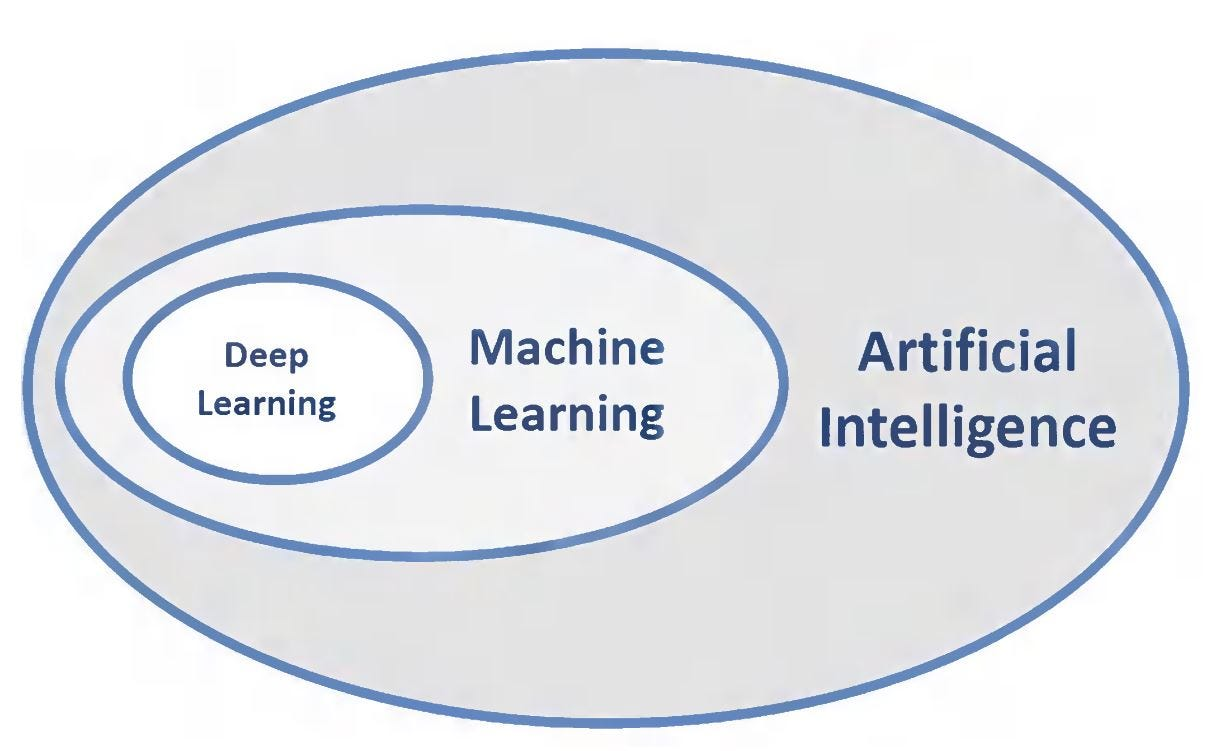
\includegraphics[width=0.6\textwidth]{imatges/preliminaries/deep-learning-family.jpg}
  \caption[Deep Learning Family]{\textit{Deep Learning Family. Illustration by Medium}}
  {\label{fig:deep-learning-family}}
\end{figure}

\section{Deep Neural Networks}

Deep neural networks are part of the deep learning algorithms within the realm
of machine learning, which, as mentioned earlier, falls under the umbrella of
artificial intelligence. is an
illustration of the deep learning family. \\


Deep neural networks, also known as fully connected layers (Figure
\ref{fig:deep-nn}), are modeled after the human brain. These algorithms achieve
their functionality by propagating signals from the input layer to the output
layer while passing through intermediate hidden layers. Each layer consists of
neurons responsible for detecting patterns from the incoming connections. These
neurons perform a crucial task by combining input from the data with a
corresponding set of coefficients, also known as weights. These weights act as
amplifiers or dampeners, modulating the impact of the input on the neuron's
activation. \\

By leveraging this mechanism, each layer in the deep neural network acquires
the capability to capture distinctive features from the input data. Notably, as
the signal travels deeper into the network, the extracted features become
increasingly sophisticated and abstract. This characteristic arises from the
hierarchical nature of the network architecture, enabling the model to learn
and discern intricate patterns and representations. \\

The process of feature extraction in deep neural networks allows the network to
progressively learn and uncover complex relationships within the data. As the
signal traverses through the network's layers, each subsequent layer builds
upon the extracted features from the previous layer, resulting in the
generation of more intricate and comprehensive representations. This ability to
capture and model hierarchical features is a significant advantage of deep
neural networks, making them particularly effective in tasks requiring the
recognition of complex patterns and high-level abstractions.

\begin{figure}[H]
  \centering
  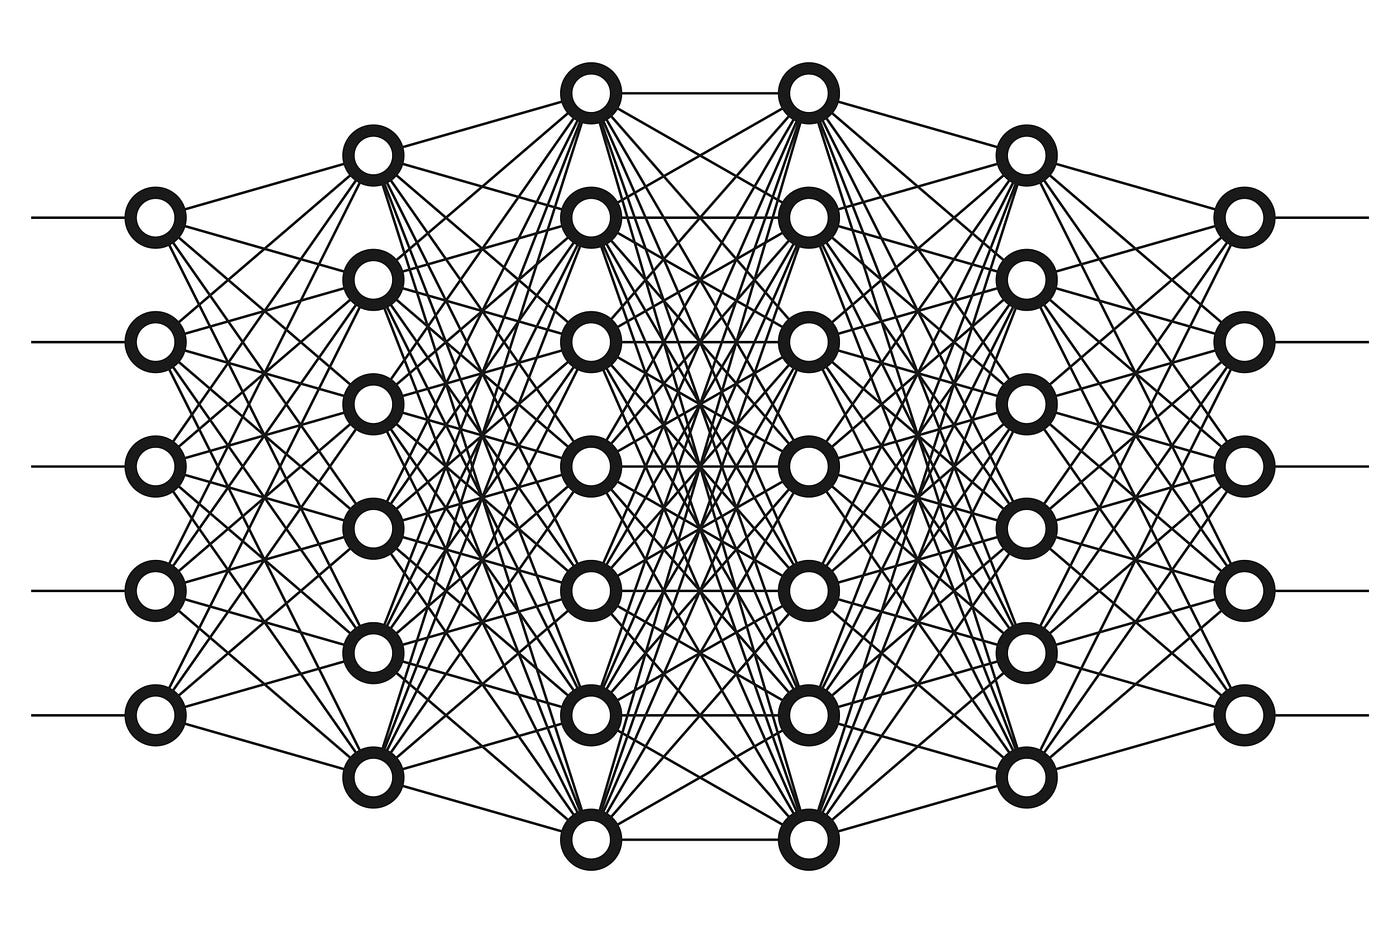
\includegraphics[width=0.6\textwidth]{imatges/preliminaries/deepnn.jpg}
  \caption[Deep Neural Network] {\textit{Deep Neural Network.
  Illustration by Medium}}
  {\label{fig:deep-nn}}
\end{figure}

The minimum unit in a layer is known as a perceptron or neuron, which bears a
resemblance to human neurons (Figure \ref{fig:perceptron}). The perceptron was
created by Frank Rosenblatt in 1958 and it is the oldest form of a simple
neural network. \\

Each perceptron in the network has an associated value that is computed based
on the incoming nodes and edges. The computation occurs as follows: the
products of inputs and their respective weights are summed with a bias, and
this sum then passes through the node's activation function. The purpose of the
activation function is to compress the resulting value within the range of 0 to
1, introducing non-linearity and enabling the model to learn complex
relationships within the data. The resultant value determines the extent to
which the signal should propagate through the network, thus influencing the
final outcome.


\begin{figure}[H]
  \centering
  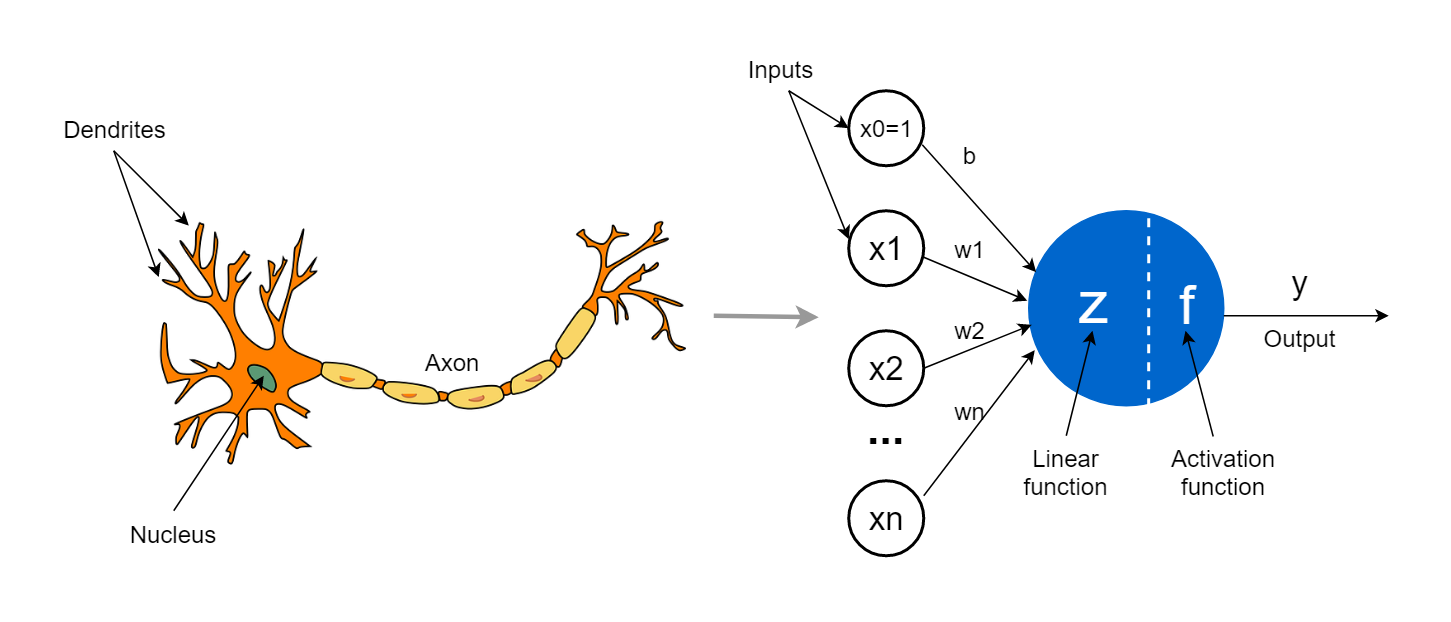
\includegraphics[width=0.8\textwidth]{imatges/preliminaries/perceptron.png}
  \caption[The Perceptron]{\textit{The Perceptron. Illustration by Medium}}
  {\label{fig:perceptron}}
\end{figure}

\newpage

\section{Convolutional Neural Networks}

A convolutional neural network (CNN) is a specific type of neural network that
is particularly well suited for analyzing images. One of the key innovations of
CNNs is their ability to automatically learn a large number of filters in
parallel. These filters are learned during the training process and are
specifically tailored to solve a particular predictive modeling problem, such
as image classification. By learning these filters, CNNs become adept at
extracting relevant features and patterns from visual data without the need for
manual feature engineering. \\

CNNs are designed to learn spatial hierarchies of features through a process
called back-propagation. During training, the network adapts its internal
parameters, or weights, by iteratively propagating the error backwards from the
output to the input layers. This allows the network to gradually adjust its
weights in a way that minimizes the difference between its predicted outputs
and the true outputs. \\

One key distinction of CNNs compared to regular neural networks is their use of
parameter sharing. In a CNN, all neurons within a particular feature map share
the same weights. This sharing of weights significantly reduces the number of
parameters in the network, making it more computationally efficient. By sharing
weights, the network can detect the same patterns or features regardless of
their spatial position in the input data. This property, known as translation
invariance, enables CNNs to recognize objects or patterns regardless of their
location within an image.\\

To build a CNN, we need four main types of layers:

\begin{itemize}
  \item Convolutional Layers
  \item Pooling Layers
  \item Fully Connected Layers
  \item Non-linearity Layers
\end{itemize}

\subsection{Convolutional Layers}

A convolutional layer (Figure \ref{fig:convolutional-layer}) is
responsible for detecting and extracting features from the input data. It
consists of a set of learnable filters, also known as kernels or feature
detectors. Each filter is a small matrix of weights that convolves
across the input data to perform a dot product operation at each spatial
location.  \\

The filter convolves across the input data with a defined stride,
which specifies the amount of shift between each position. At each spatial
location, a dot product is computed between the filter and the overlapping
region of the input. The dot product involves element-wise multiplication of
the filter values with the corresponding input values, followed by summing up
the results. \\

The result of each dot product operation is a single value, forming a pixel in
the output feature map. Additionally, an activation function is applied
element-wise to introduce non-linearity into the network.

\begin{figure}[H] \centering
  \begin{adjustbox}{width=0.75\textwidth, trim={0cm 0cm 0cm 0.35cm}, clip}
  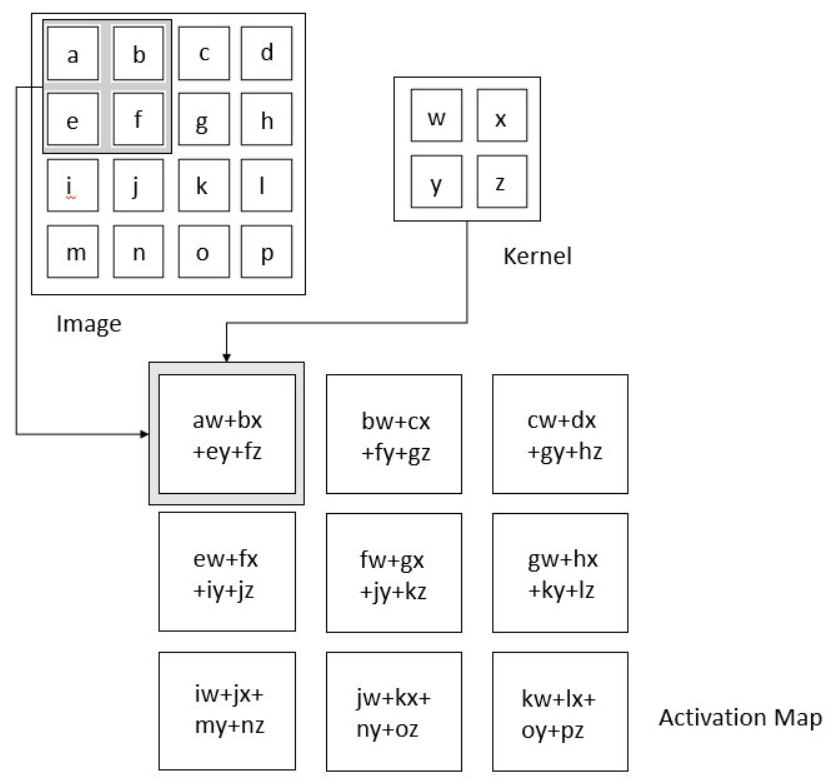
\includegraphics[]{imatges/preliminaries/convolutional-layer.png}
  \end{adjustbox}
  \caption[Convolutional Operation on Input]{\textit{Convolutional
  Operation on Input. Illustration by towardsdatascience}}
{\label{fig:convolutional-layer}} \end{figure}

\newpage

\subsection{Pooling Layers}

A pooling layer (Figure \ref{fig:pooling-layer}) performs a
summarizing of nearby outputs in the network, effectively replacing certain
locations with a condensed representation. This reduces the spatial
dimensionality of the output, leading to decreased computational requirements
and weight parameters. The pooling operation is applied independently to each
slice of the representation. \\

Various pooling functions exist, including averaging the values within a
rectangular neighborhood, computing the L2 norm of the neighborhood, or using a
weighted average based on distance. However, the most widely used method is max
pooling, which selects the maximum output value from the neighborhood.

\begin{figure}[H]
  \centering
  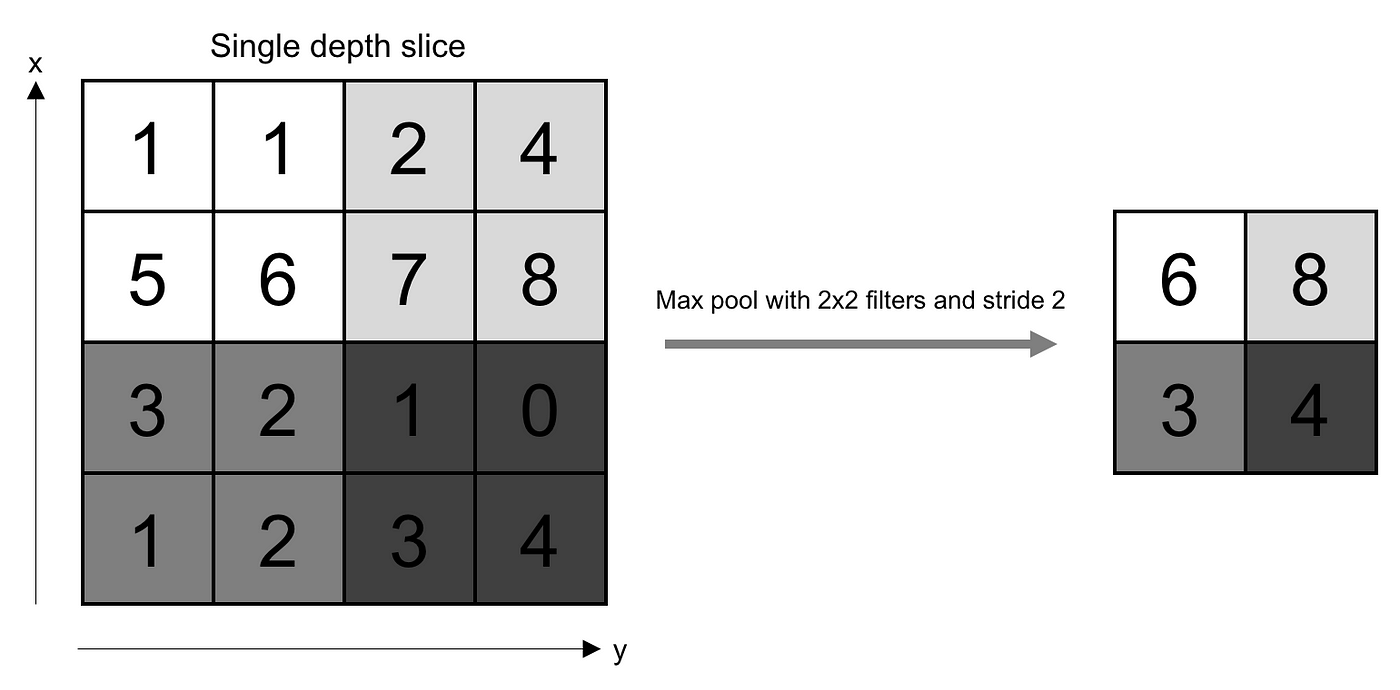
\includegraphics[width=0.8\textwidth]{imatges/preliminaries/polling-layer.png}
  \caption[Max Polling Operation on Input]{\textit{Max Polling Operation on Input. Illustration by towardsdatascience}}
  {\label{fig:pooling-layer}}
\end{figure}

\subsection{Fully Connected Layers}

Neurons in this layer have full connectivity with all neurons in the preceding
and succeeding layer. This is why it can be computed as usual by a matrix
multiplication followed by a bias effect. The topology in the fully connected
portion of a CNN depends on various factors, including the complexity of the
task, the nature of the data, and the capacity of the model. There is no fixed
rule for determining the exact number of neurons or layers, and it often
requires experimentation and tuning. \\

A fully connected layer (Figure \ref{fig:deep-nn}), helps to map the
representation between the input and the output.

\subsection{Non-linearity Layers}

Convolutional operations in neural networks are linear, meaning they capture
linear patterns in the data. However, many objects in images exhibit non-linear
characteristics that cannot be effectively detected using linear operations
alone. To address this limitation, non-linearity layers, such as activation
functions, are typically applied immediately after the convolutional layer.
These non-linearity layers may introduce non-linear transformations to the
activation maps, enabling the network to learn and detect complex, non-linear
patterns in the data. \\

There are many types of non-linearity functions applied after the convolutional
layers, the most popular are: \\

\begin{itemize}

  \item \textbf{Sigmoid}

    The sigmoid function takes a real-valued number and “squashes” it into a
    range between 0 and 1.

    \centering {
      \begin{tikzpicture}
        \draw[->] (-5,0) -- (5,0) node[right] {$x$};
        \draw[->] (0,-0.5) -- (0,1.5) node[above] {$\sigma(x)$};
        \draw[domain=-5:5, smooth, variable=\x, blue] plot (\x, {1/(1 + exp(-\x))});
        \draw[dashed] (-5, 0.0) node[left] {0};
        \draw[dashed] (-5, 1) node[left] {1} -- (5, 1);
      \end{tikzpicture}
    }

    \raggedright
    Mathematically, the sigmoid function is expressed as:

    \[ \sigma(x) = \frac{1}{1 + e^{-x}} \]

    \newpage

  \item \textbf{ReLU}

    The Rectified Linear Unit (ReLU) is maybe the most popular activation
    functions in the last few years. The function is just simply threshold at
    zero.

    \centering \begin{tikzpicture} \draw[->] (-5,0) -- (5,0) node[right]
      {$x$}; \draw[->] (0,-0.5) -- (0,5) node[above] {$\text{ReLU}(x)$};
      \draw[domain=-5:0, smooth, variable=\x, blue] plot (\x, 0);
      \draw[domain=0:5, smooth, variable=\x, blue] plot (\x, \x);
      \draw[dashed] (-5, 0.0) node[left] {0}; \draw[dashed] (-5, 1) node[left]
    {1} -- (5, 1); \end{tikzpicture}

    \raggedright
    Mathematically, the ReLU function is expressed as:

    \[f(x) = \max(0, x)\]

  \item \textbf{Tanh}

    The hyperbolic tangent function tanh compresses a real-valued number to
    the range of [-1, 1]. Similar to the sigmoid function, tanh exhibits
    saturation, but unlike sigmoid, its output is centered around zero.

    \centering
    \begin{tikzpicture}
      \draw[->] (-5,0) -- (5,0) node[right] {$x$};
      \draw[->] (0,-1.5) -- (0,1.5) node[above] {$\tanh(x)$};
      \draw[domain=-5:5, smooth, variable=\x, blue] plot (\x, {tanh(\x)});
      \draw[dashed] (-5, -1) node[left] {-1} -- (5, -1);
      \draw[dashed] (-5, 1) node[left] {1} -- (5, 1);
    \end{tikzpicture}

    \raggedright
    Mathematically, the tanh function is expressed as:

    \[ \tanh(x) = \frac{{e^x - e^{-x}}}{{e^x + e^{-x}}} \]

\end{itemize}

\section{Loss Function}

A loss function, also known as a cost function or an objective function, is a
measure used in machine learning and optimization algorithms to quantify how
well a model performs on a given task. It measures the discrepancy between
the predicted outputs of a model and the true values or labels associated with
the training data. \\

Different machine learning tasks and algorithms may use different loss
functions, depending on the specific problem being addressed. Commonly used
loss functions include:

\begin{itemize}
  \item Mean Squared Error (MSE)
  \item Binary Cross-Entropy
  \item Mean Absolute Error (MAE)
  \item Cross-entropy Loss
\end{itemize}

For this thesis, the loss function used to train the models is
Cross-entropy Loss as this is a multiclass problem. Do not confuse the
optimizer algorithm with the metric used to evaluate how good models are. We
used the ROC AUC with one-vs-rest strategy to evaluate the models performance,
explained in Section \ref{sec:metrics}. \\

Cross-entropy loss, also known as log loss, is a widely used loss function in
machine learning, particularly in classification tasks. It measures the
dissimilarity between predicted class probabilities and true class labels.
\\

In multi-class classification, the cross-entropy loss is calculated using the
true class labels \(y\) and the predicted class probabilities \(p\) for each
class. It can be defined as:

\[-\sum_{i=1}^{C} y_i \log(p_i)\]

\noindent where:

\begin{itemize}
  \item \(C\) is the total number of classes.
  \item \(y_i\) represents the true label for class \(i\).
  \item \(p_i\) represents the predicted probability for class \(i\).
\end{itemize}

\section{Metrics}
{\label{sec:metrics}}

There are various metrics commonly used to assess the quality of a model's predictions.
In this section, we present a selection of metrics that we find relevant for evaluating our models.

\subsection{Confusion Matrix}

A confusion matrix (Figure \ref{fig:confusion-matrix}) is a square matrix with dimensions  NxN,
where  N represents the total number of classes being predicted.
It provides a visual representation of the errors or confusion made by a classification
model during its predictions. \\


\begin{figure}[H]
  \begin{adjustbox}{trim={0pt 0.5cm 0pt 1cm}, clip}
    \centering
    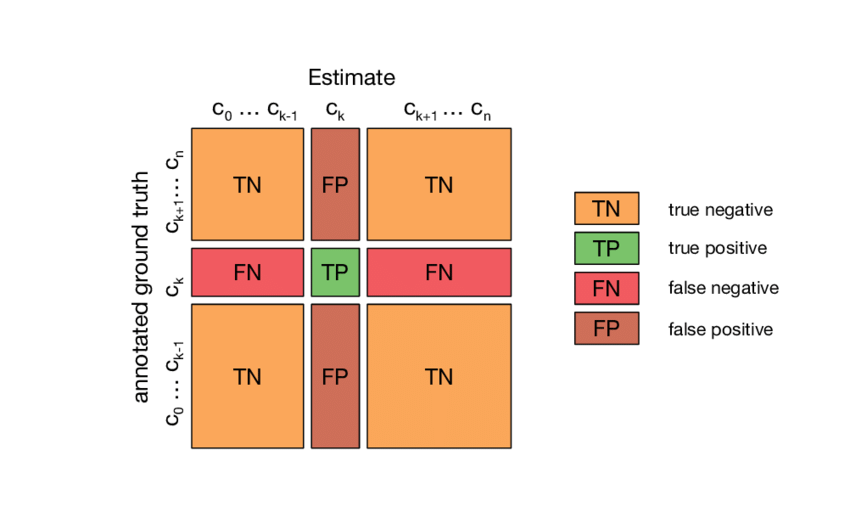
\includegraphics[width=0.9\textwidth]{imatges/preliminaries/confusion-matrix.png}
  \end{adjustbox}
  \caption[Confusion Matrix Multi-Class]{\textit{Confusion Matrix Multi-Class. Illustration by kaggle}}
  {\label{fig:confusion-matrix}}
\end{figure}

From confusion matrix we can obtain other metrics such as:

\begin{itemize}
  \item \textbf{True Positive (TP)}

    This refers to an outcome where the model accurately predicts the positive class.
  \item \textbf{False Positive (FP)}

    This describes a situation where the model mistakenly predicts the positive class when it should have predicted the negative class.
  \item \textbf{True Negative (TN)}

    This represents an outcome where the model correctly predicts the negative class.
  \item \textbf{False Negative (FN)}

    This indicates a scenario where the model incorrectly predicts the negative class instead of predicting the positive class.

\end{itemize}


In a logical sense, when we add up the elements on the main diagonal of the
confusion matrix, we obtain the total number of correct predictions.
Utilizing the confusion matrix values, we can compute
additional metrics such as accuracy, recall and others.

\subsection{Accuracy}

Accuracy is a commonly employed and straightforward performance metric in
classification tasks. It calculates the ratio of correct predictions to the
total number of predictions made on a dataset, thus determining the likelihood
of correctly classifying an input. Accuracy is especially valuable when working
with a balanced dataset, where the number of instances in each class is roughly
equivalent.

\[Accuracy = \frac{TP + TN}{TP + TN + FP + FN}\]

\subsection{TPR}

TPR stands for True Positive Rate, and it is also known as sensitivity or
recall. It measures the proportion of actual positive cases that are correctly
identified as positive by a classification model or test.

\[
  \text{TPR} = \frac{\text{TP}}{\text{TP} + \text{FN}}
\]

\subsection{FPR or Recall}

FPR stands for False Positive Rate, and it measures the proportion of actual
negative cases that are incorrectly identified as positive by a classification
model or test.

\[ \text{FPR} = \frac{\text{FP}}{\text{FP} + \text{TN}} \]

\subsection{AUC-ROC}

The ROC Curve, when computed with the one-vs-rest (OvR) strategy for
multi-class classification, provides insights into how well the model can
differentiate a class from the rest of the classes. It is a probabilistic curve
that plots the true positive rate (TPR) against the false positive rate (FPR).
By treating the target class as the positive class and the remaining classes as
the negative class in separate binary classification tasks (\textit{Figure
\ref{fig:auc-roc}}). \\

The area under the curve (AUC) is a value between 0 and 1 that measures the
ability of a classifier to distinguish between classes. It is used as a summary
of the ROC curve. The higher the AUC, the better the performance of the model
at distinguishing between the positive and negative classes.

\begin{figure}[H]
  \centering
  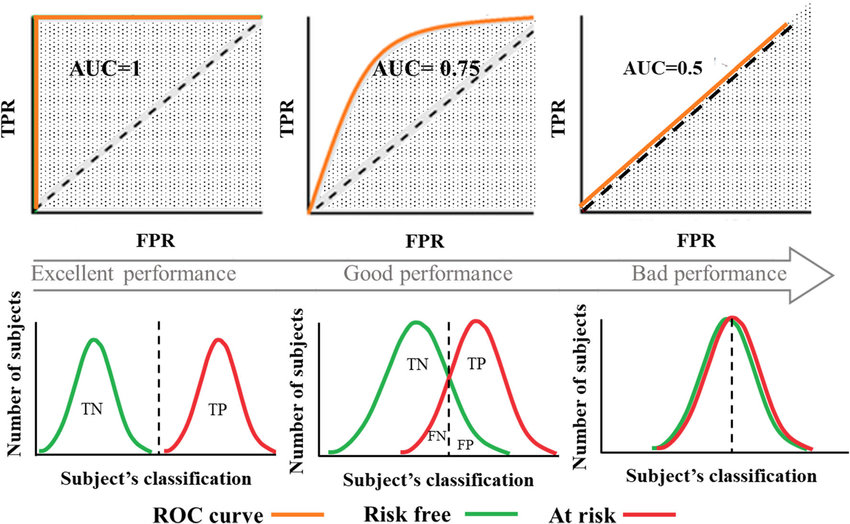
\includegraphics[width=0.7\textwidth]{imatges/preliminaries/auc.png}
  \caption[AUC-ROC Performance]{\textit{AUC-ROC Performance. Illustration by Elizabeth Louise Thomas}}
  {\label{fig:auc-roc}}
\end{figure}

\newpage

\section{Optimizer}

An optimizer is an algorithm that finds the value of the parameters (weights)
that minimize the error when mapping inputs to outputs. While training a deep
learning models, the optimizer modifies the weights of the model in each epoch
to minimize the loss function. \\

The are a considerable amount of different optimizer algorithms out there with
their pros and cons. In this section we present the family of optimizers based
on Gradient Descent optimization. This family of optimizer algorithms were used
for the thesis. \\

\subsection{Gradient Descent}

Using the Gradient Decent (SD) optimization algorithm (Figure
\ref{fig:optimization}), the weights are updated incrementally after each
epoch. The magnitude and direction of the weight update is computed by taking a
step in the opposite direction of the cost gradient. \\

Given the following defintions:

\begin{itemize}
  \item \(\Delta w\) represents the weights update.
  \item \(\eta\) (eta) denotes the "learning rate", which controls the step size of the update.
  \item  \(\frac{\partial J}{\partial w_i}\) represents the partial derivative of the cost function \(J\) with respect to the weight \(w_i\).
  \item \(\nabla J(w)\) represents the gradient of the cost function \(J(w)\) with respect to the weights \(w\).
\end{itemize}

We could compute the weight update after each epoch with the following
mathematical expression:

\[\nabla J(w) = (\frac{\partial J}{\partial w_1}, \frac{\partial J}{\partial w_2}, \ldots, \frac{\partial J}{\partial w_n})\]

\[
  \Delta w = -\eta \cdot \nabla J(w)
\]


\[
  w = w + \Delta w
\]



In Gradient Descent optimization, we compute the cost gradient based on the
complete training set, in case of very large datasets, using Gradient Descent
can be quite costly since we are only taking a single step for one pass over
the training set – thus, the larger the training set, the slower our algorithm
updates the weights and the longer it may take until it converges to the global
cost minimum. \\

A high level pseudo-implementation of the Gradient Descent algorithm: \\

\begin{itemize}[label=\(\circ\)]
  \item for each epoch:
    \begin{itemize}[label=\(\circ\), topsep=0pt]
      \item for each weight \(j\):
        \begin{itemize}[label=\(\circ\), topsep=5pt]
          \item \(w_j = w_{j-1} + \Delta w_j\)
        \end{itemize}
    \end{itemize}
\end{itemize}

\begin{figure}[H]
  \centering
  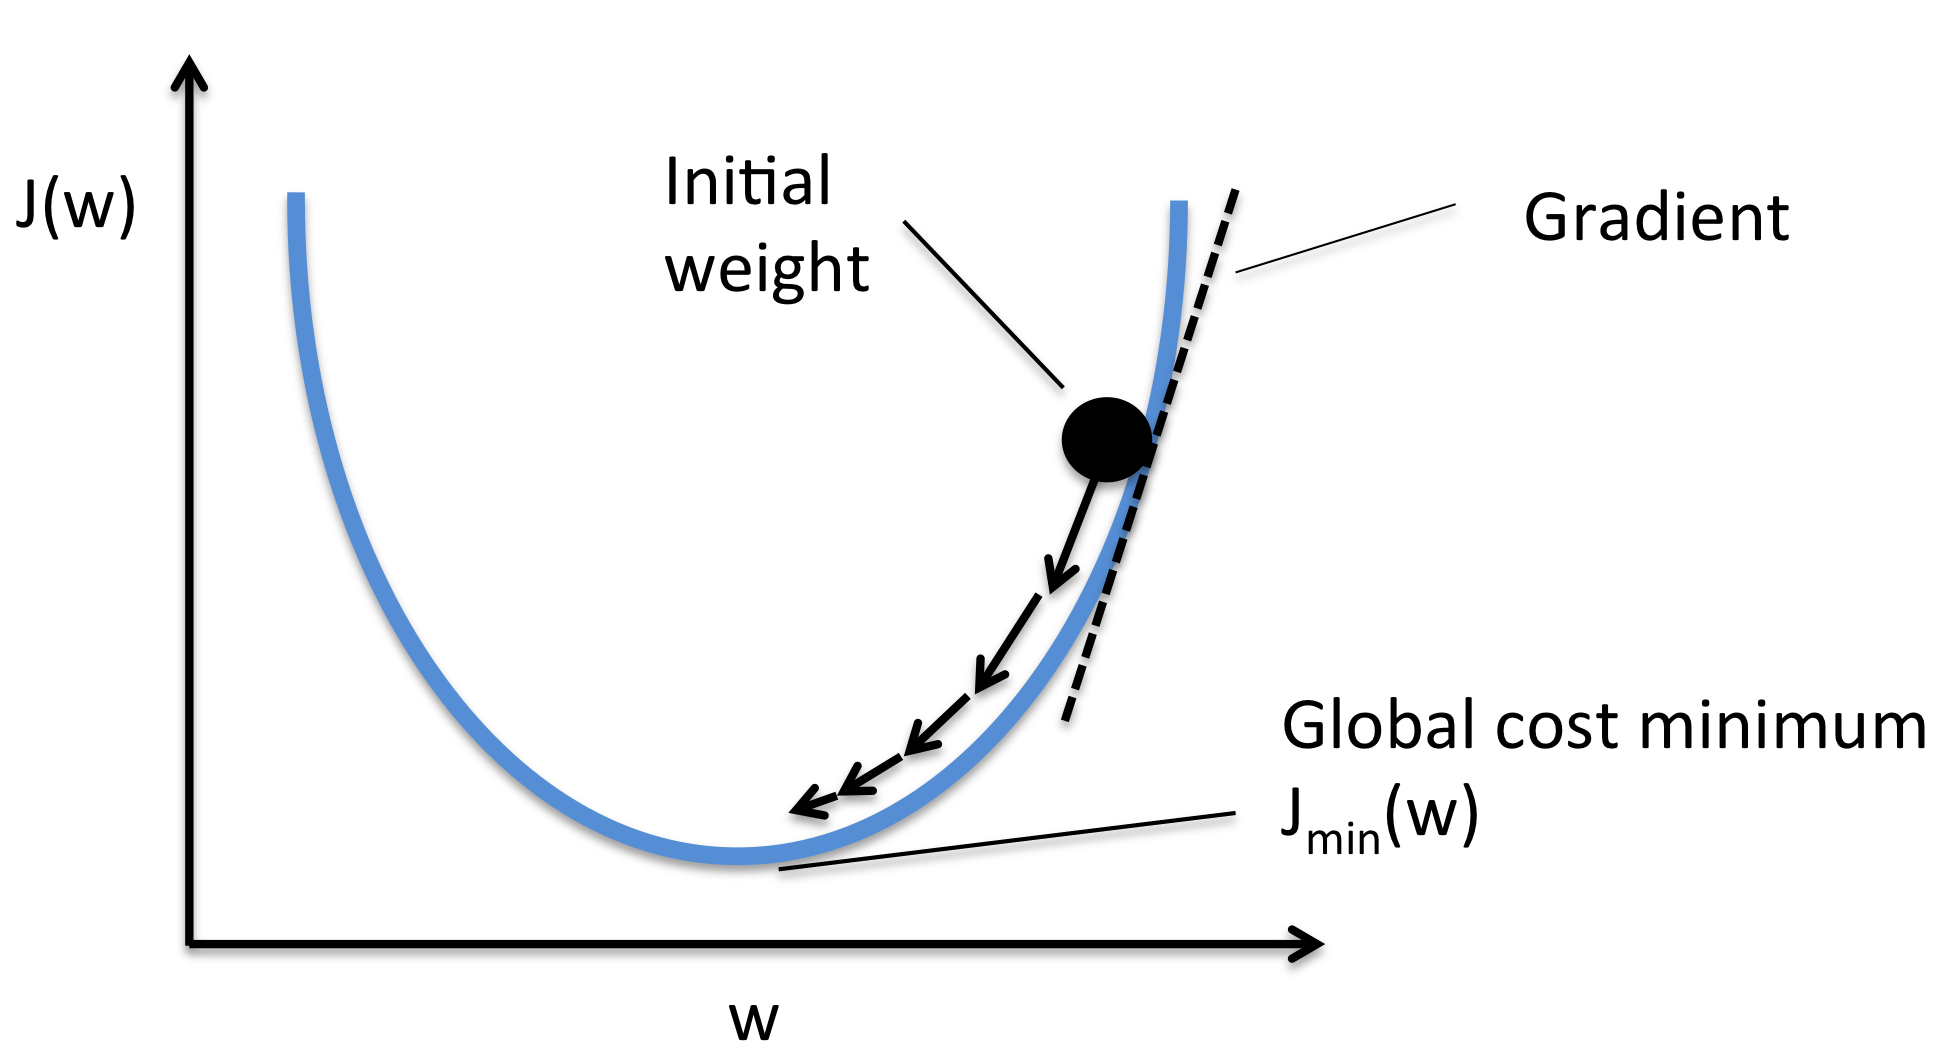
\includegraphics[width=0.5\textwidth]{imatges/preliminaries/optimization.png}
  \caption[Optimization Using Gradient Descent]{\textit{Optimization Using Gradient Descent. Illustration by raschka}}
  {\label{fig:optimization}}
\end{figure}

\newpage

\subsection{Stochastic Gradient Descent}

Stochastic Gradient Descent (SGD) work similar to the Gradient Descent but the
weight updates are not accumulated as we have seen above for Gradient Descent.
Instead, the weights are updated after each training sample. Due to its
stochastic nature, the path towards the global cost minimum is not “direct” as
in Gradient Descent, but may go “zig-zag”if we are visualizing the cost surface
in a 2D space, see Figure \ref{fig:sgdvsgd}. However, it has been shown that
Stochastic Gradient Descent almost surely converges to the global cost minimum
if the cost function is convex. \\

A high level pseudo-implementation of the Stochastic Gradient Descent
algorithm:

\begin{itemize}[label=$\circ$]
  \item for each epoch or until approx. cost minimum is reached:
    \begin{itemize}[label=$\circ$, topsep=0pt]
      \item for training sample \(i\):
        \begin{itemize}[label=$\circ$, topsep=5pt]
          \item for each weight \(j\):
            \begin{itemize}[label=$\circ$, topsep=10pt]
              \item \(w_j = w_{j-1} + \Delta w_j\), where \(\Delta w_j = \eta (target^{(i)} - output^{(i)})x_{j}^{(i)}\)
            \end{itemize}
        \end{itemize}
    \end{itemize}
\end{itemize}

\begin{figure}[H]
  \centering
    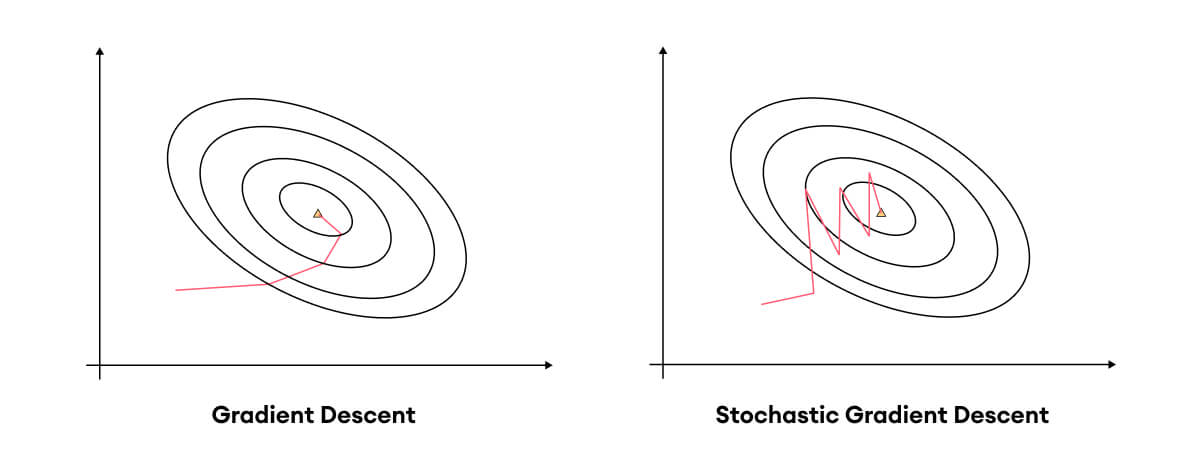
\includegraphics[width=0.8\textwidth]{imatges/preliminaries/sgdvsgd.jpeg}
  \caption[GD vs SGD]{\textit{GD vs SGD. Illustration by superannotate}}
  {\label{fig:sgdvsgd}}
\end{figure}

\newpage

\section{Forward and Backward Propagation}

Forward and back-propagation are fundamental processes in training neural
networks and optimizing their parameters. They play a crucial role in enabling
the network to learn from data and improve its performance over time. \\

Resuming the forward-propagation and back-propagation (\textit{Figure
\ref{fig:forward-and-back-propagation}}), in order to find the direction of the
steepest descent (minimising the overall loss function), we need to calculate
gradients of the loss function with respect to weights and bias. After that,
we’ll be able to update weights and bias using negative gradients multiplied by
the learning rate.

\begin{figure}[H]
  \centering
  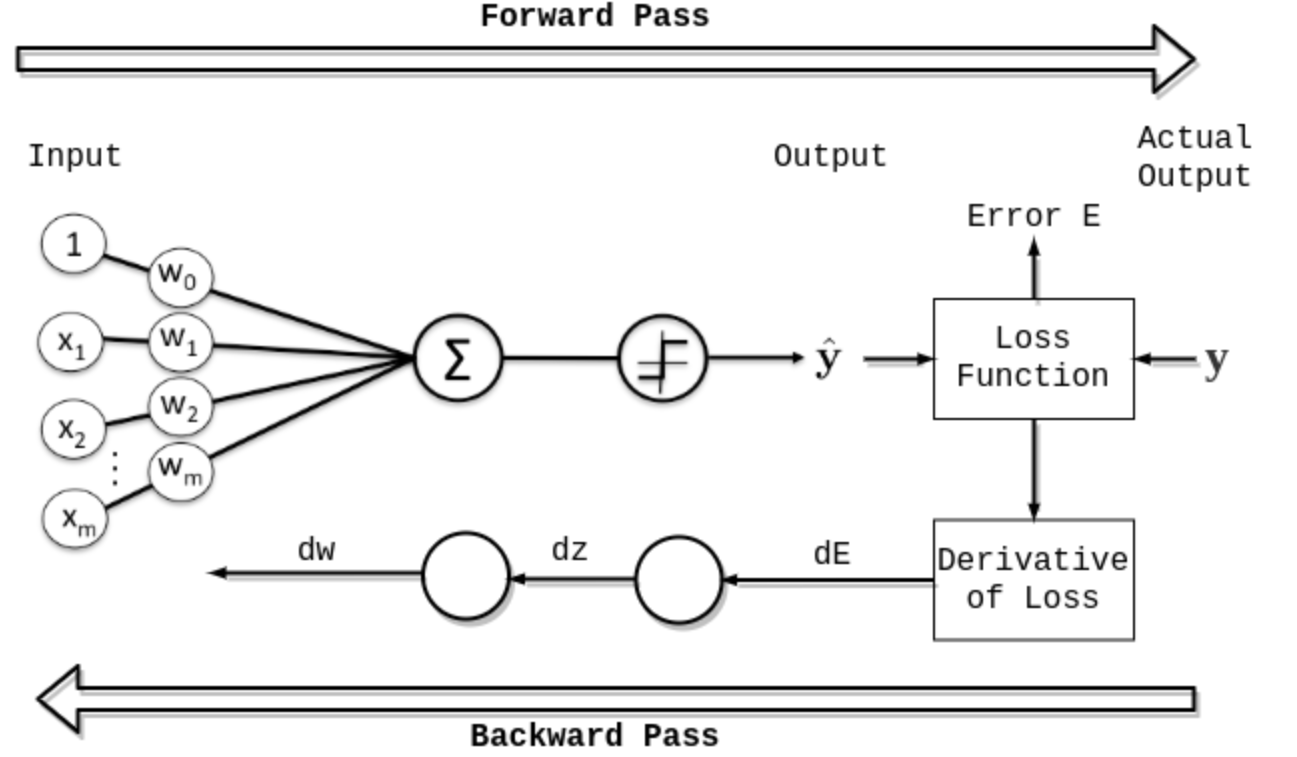
\includegraphics[width=0.8\textwidth]{imatges/preliminaries/front-and-back-prop.png}
  \caption[Forward and Backward Propagation]{\textit{Forward and Backward Propagation. Illustration by baeldung}}
  {\label{fig:forward-and-back-propagation}}
\end{figure}


\subsection{Forward Propagation}

Forward propagation refers to the process of computing the output of a neural
network given an input or a batch of inputs. During forward propagation, the
input data flows through the network's layers in a sequential manner, from the
input layer to the output layer. Each layer performs a series of computations,
typically involving linear transformations (such as matrix multiplications)
followed by activation functions. \\

As the data flows forward through the network, intermediate outputs, also known
as activations or feature maps, are computed at each layer. These activations
are then passed on as inputs to the subsequent layers until the final output is
produced. The forward propagation process essentially calculates the predicted
output of the network for a given input.

\subsection{Backward Propagation}

Backward propagation, short for backward propagation of errors, is the process
of computing the gradients of the network's parameters with respect to a loss
function. These gradients indicate the sensitivity of the network's output to
changes in its parameters and are used to update the parameters during the
training process. \\

The backward propagation algorithm starts from the final output of the network
and propagates the error gradients backward through the network's layers. It
computes the gradients layer by layer using the chain rule of calculus. The
gradients quantify how each parameter contributed to the overall error of the
network and provide information on how to adjust the parameters to reduce the
error.


\section{Under-fitting vs Over-fitting}

Under-fitting is a prevalent challenge in machine learning, occurring when the
model fails to establish a meaningful relationship between the input and target
variable. Insufficiently capturing the features of the data results in
increased errors in both the training and unseen data samples. \\

Over-fitting is also a prevalent challenge in machine learning but it is really
common in deep learning algorithms. Deep learning models try to fit the
training data entirely and ends up memorizing the data patterns and the
noise/random fluctuations. These models fail to generalize and perform well in
the case of training data, but fail in unseen data scenarios, defeating the
model's purpose.

\begin{figure}[H]
  \centering
  \begin{adjustbox}{width=\textwidth, trim={0cm 1.25cm 0cm 2.25cm}, clip}
  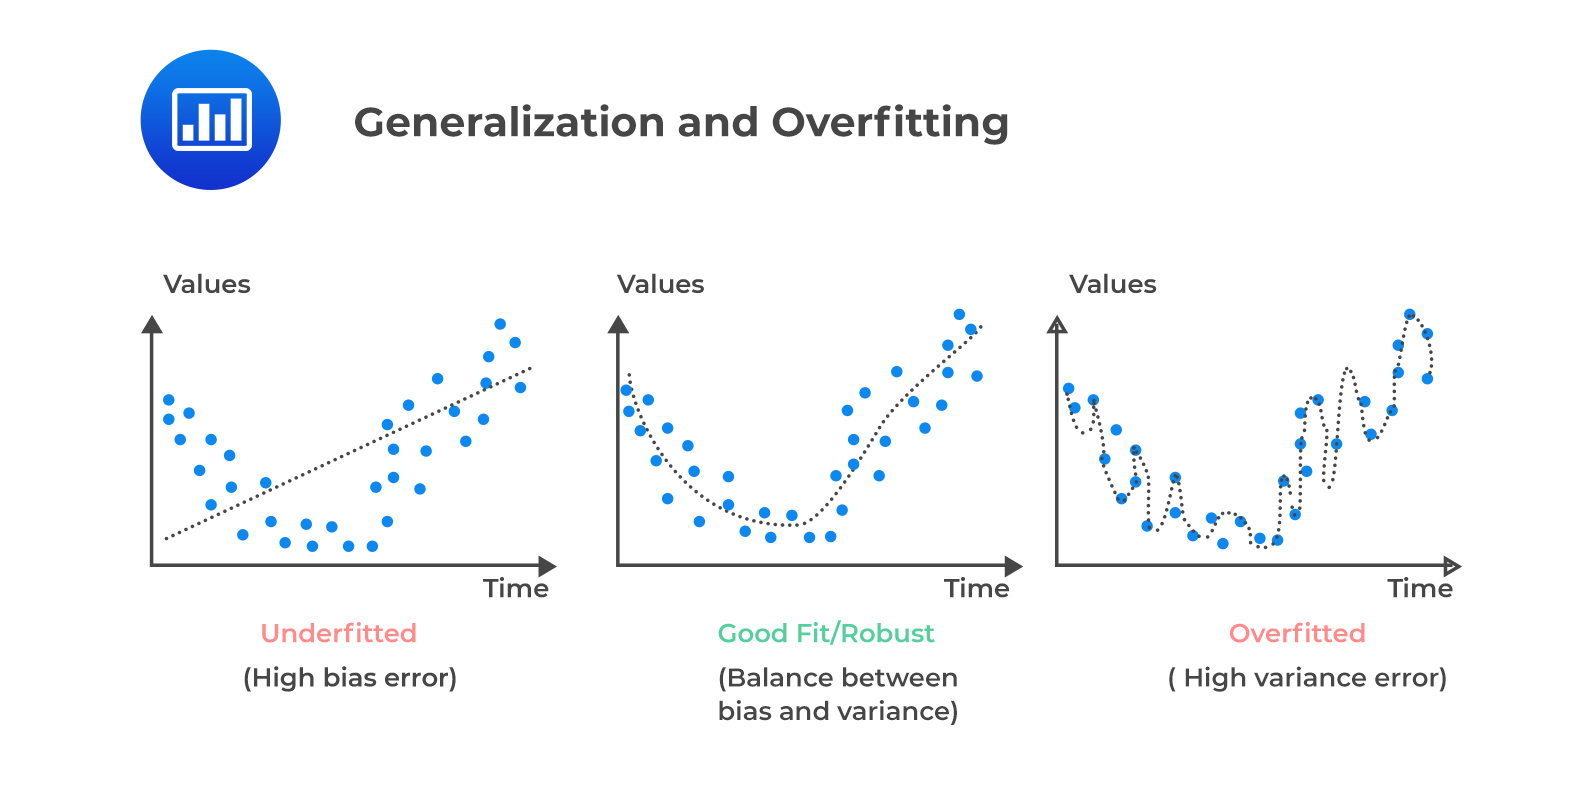
\includegraphics[width=\textwidth]{imatges/preliminaries/fit-scenes.jpg}
  \end{adjustbox}
  \caption[Fitting Scenarios]{\textit{Fitting Scenarios. Illustration by towardsdatascience}}
  {\label{fig:underfitting-overfitting-goodfitting}}
\end{figure}

\section{Strategies to Combat Over-fitting}

There are lot of strategies to combat over-fitting, in this section there is
presented only those used in the project. \\

\subsection{Early Stopping}

Early Stopping involves monitoring the model's performance on a validation
dataset during training. If the performance stops improving or starts
deteriorating, the training process is stopped early. By doing this, early
stopping helps find the optimal balance between model complexity and
generalization, ensuring the model does not become overly specialized to the
training data and does not perform well on unseen data. \\

\begin{figure}[H]
  \centering
  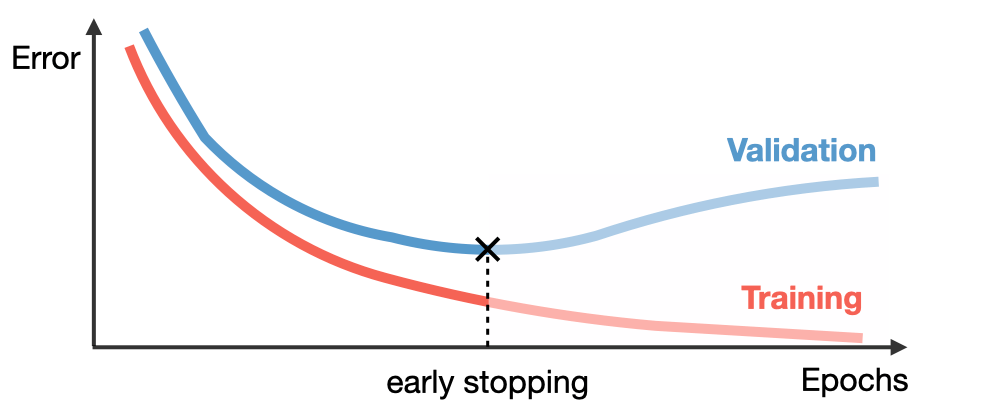
\includegraphics[width=0.7\textwidth]{imatges/preliminaries/early-stop.png}
  \caption[Early Stopping]{\textit{Early Stopping. the vertical doted line
  represents the point where the early stop mechanism should have been
  triggered. Illustration by wandb}}
  {\label{fig:early-stop}}
\end{figure}

\subsection{Learning Rate Scheduling}

The learning rate is a hyper-parameter in machine learning that determines the
step size at which a model's parameters are updated during the optimization
process. In most optimization algorithms, such as gradient descent, the
learning rate controls how quickly or slowly the model learns from the training
data. \\

There are various approaches in learning rate scheduling, below you will find
the scheduling used in the thesis.

\begin{itemize}
  \item \textbf{Learning Rate Decay}

    This learning rate scheduling works gradually reducing the learning rate
    over time or in response to certain conditions. \\

    A smaller learning rate allows the model to fine-tune its parameters more
    cautiously, preventing it from aggressively fitting to noisy or
    irrelevant patterns in the training data. A smoother or an agresive
    adjustment helps the model converge to a better generalized solution,
    reducing the risk of over-fitting. \\

    There are varius scheduler policies that we can follow to make the
    learning rate decay over the epochs. For instance, in Figure
    \ref{fig:learning-rate-decay-cosine-annealing} follows the
    Cosine Annealing Learning Rate scheduler, yet Figure
    \ref{fig:learning-rate-decay-step} follows the Step Learning
    Rate scheduler.

    \begin{figure}[H] \centering
      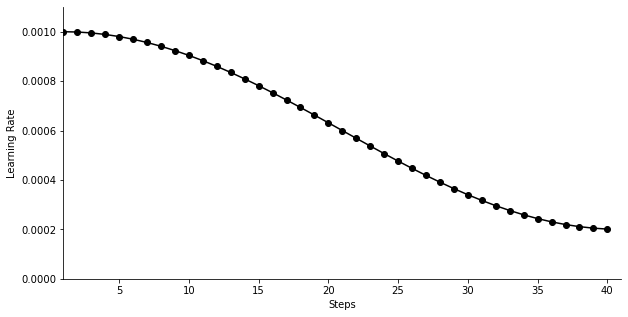
\includegraphics[width=0.6\textwidth]{imatges/preliminaries/cosinus-scheduler.png}
      \caption[Cosine Annealing Learning Rate Scheduler]{\textit{Cosine
      Annealing Learning Rate Scheduler. A learning rate decay scheduler with
      smoother behavior. }}
    {\label{fig:learning-rate-decay-cosine-annealing}} \end{figure}

    \begin{figure}[H] \centering
      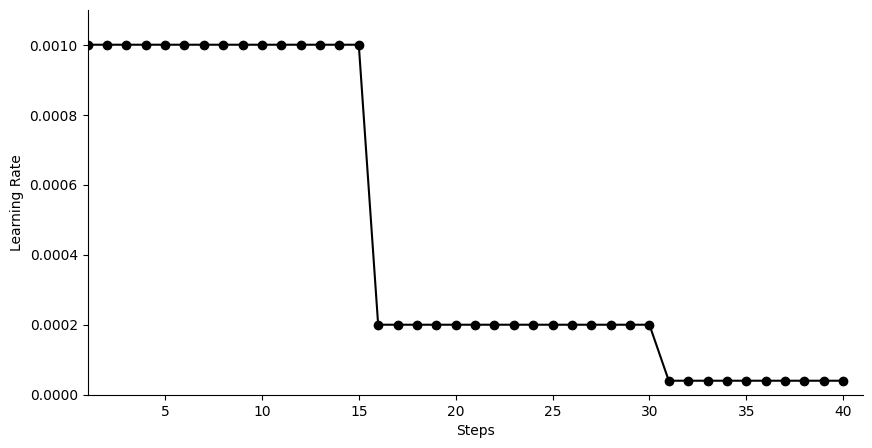
\includegraphics[width=0.6\textwidth]{imatges/preliminaries/step-scheduler.png}
      \caption[Step Learning Rate Scheduler]{\textit{Step Learning Rate
      Scheduler. A learning rate decay scheduler with and agresive behavior.
      }} {\label{fig:learning-rate-decay-step}}
    \end{figure}

    \newpage

  \item \textbf{Cycling Learning}

    Cyclic learning rate scheduling is popular for faster convergence and
    improved generalization. By cycling the learning rate, models explore
    diverse loss landscape regions, escaping local minima for better optima.
    Variations like triangular and cosine annealing alternate or smoothly
    transition between lower and upper bounds. This approach adds variation
    and exploration to optimization, enhancing model performance and
    convergence. \\

    As well as in learning rate decay, there are various scheduler with it's
    own policy. Figure \ref{fig:cycling-rate-decay} is a
    representation of a Cosine Annealing Warm Restart scheduler.
    \begin{figure}[H] \centering
      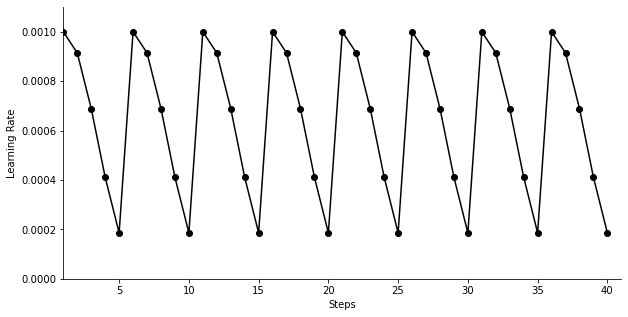
\includegraphics[width=0.6\textwidth]{imatges/preliminaries/CosineAnnealingWarmRestarts-scheduler.png}
      \caption[Cosine Annealing Warm Restart]{\textit{Cosine Annealing Warm
      Restart. A cosinus cycling learning scheduler.}}
    {\label{fig:cycling-rate-decay}} \end{figure} \end{itemize}

\newpage

\subsection{Dropout}

Dropout is a regularization method \cite{DropoutPaper}. The idea behind dropout
is to prevent over-fitting and improve generalization in neural networks by
randomly "dropping out" or deactivating a fraction of the neurons during
each training iteration. \\

By randomly dropping out neurons, the network becomes more robust and less
sensitive to the precise configuration of any single neuron. It forces the
network to learn redundant representations and prevents co-adaptation.

\begin{figure}[H]
  \centering
  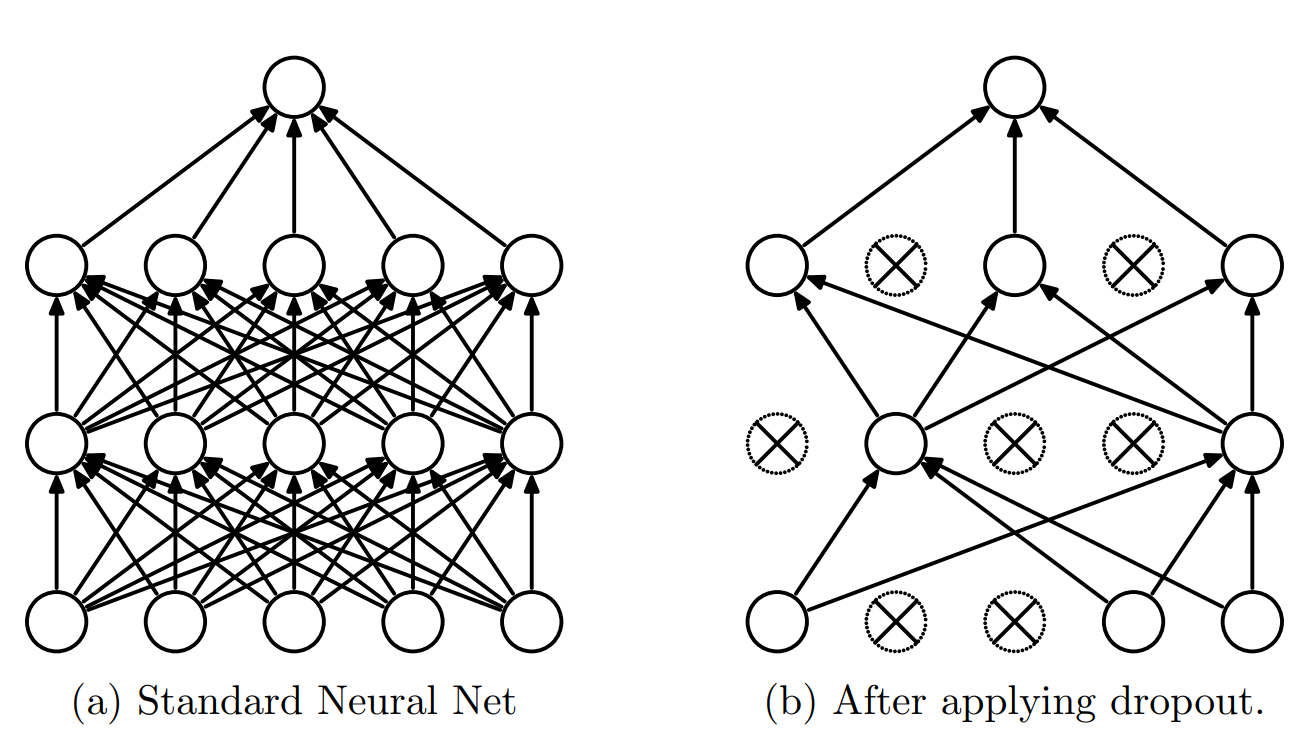
\includegraphics[width=10cm]{imatges/preliminaries/dropout.png}
  \caption[Dropout]{\textit{Dropout Neural Net Model. \textbf{Left}: A standard neural net with 2 hidden layers. \textbf{Right}:
  An example of a thinned net produced by applying dropout to the network on the left.
  Crossed units have been dropped. Illustration by Srivastava}}
  {\label{fig:dropout}}
\end{figure}

\newpage

\subsection{Data Augmentation}

Data augmentation encompasses various techniques utilized to expand the dataset
by introducing modifications, thereby increasing the number of examples. Its
purpose is not only to enlarge the dataset but also to enhance its diversity.
By acting as a regularization, data augmentation aids in mitigating
over-fitting during machine learning model training.

\begin{figure}[H]
  \centering
  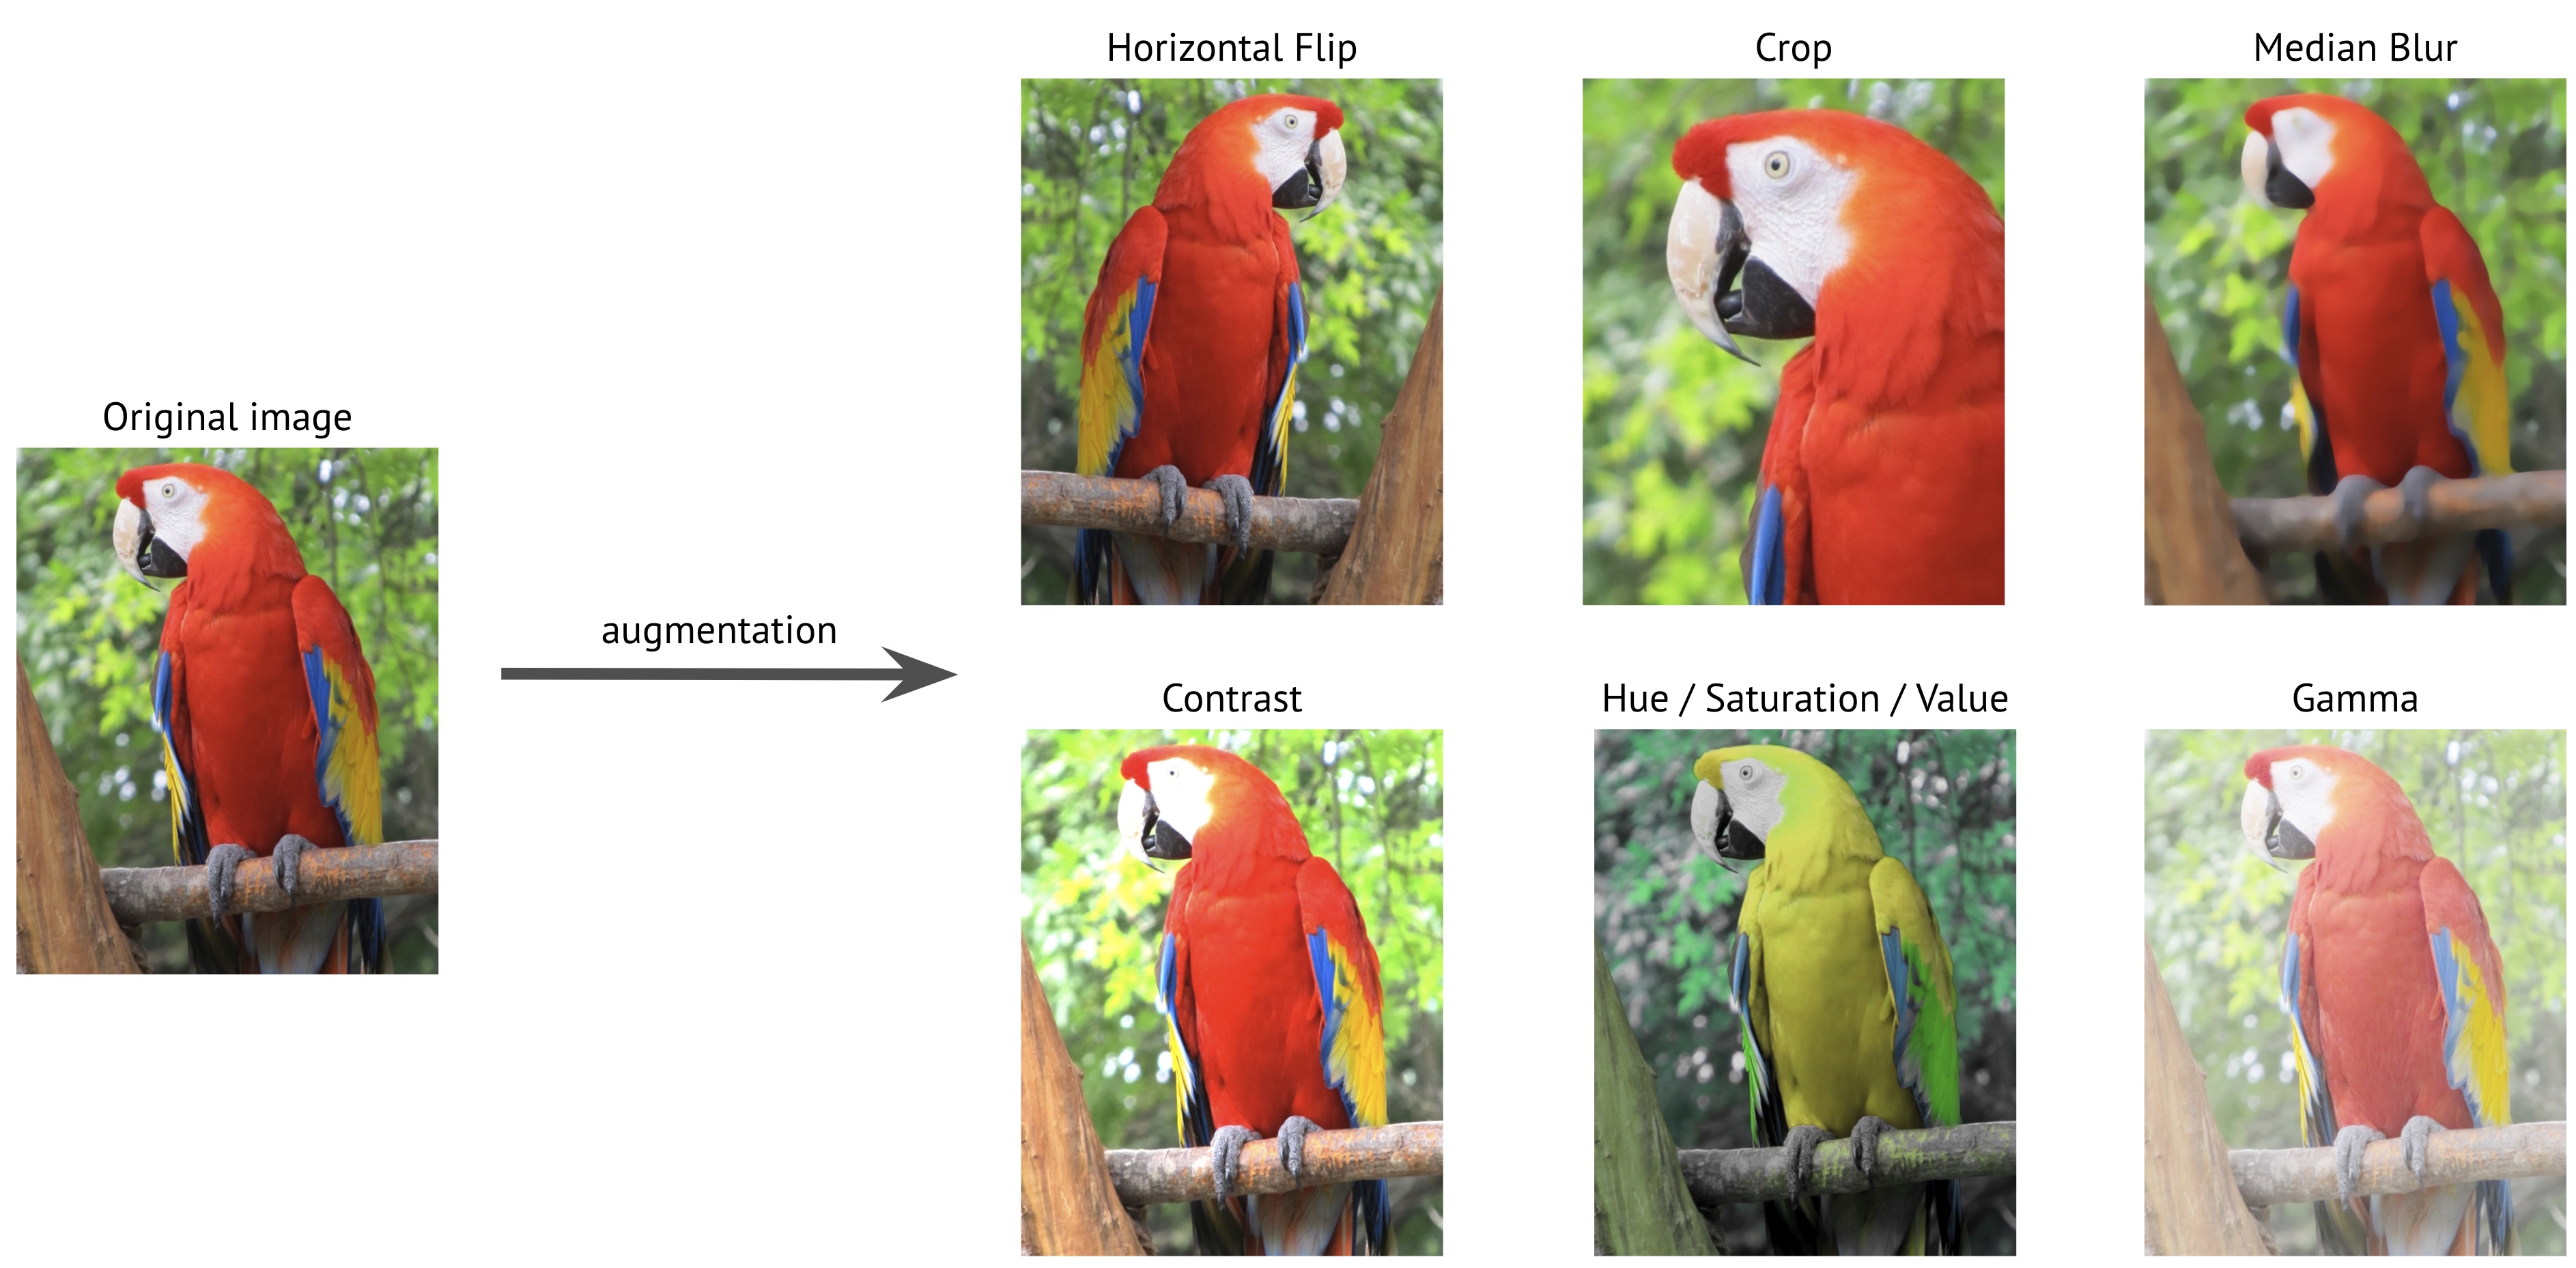
\includegraphics[width=0.7\textwidth]{imatges/preliminaries/augmentation.jpg}
  \caption[Data Augmentation]{\textit{Data Augmentation. Illustration by Albumentations}}
  {\label{fig:augmentation}}
\end{figure}


\section{Train, Validation and Test Sets}

The primary method employed to validate the models involves dividing the
original dataset into three subsets using the Holdout set scheme (Figure
\ref{fig:holdout-test-scheme}).

\begin{figure}[H]
  \centering
  \begin{adjustbox}{width=0.8\textwidth, trim={0cm 0.5cm 0cm 0.5cm}, clip}
    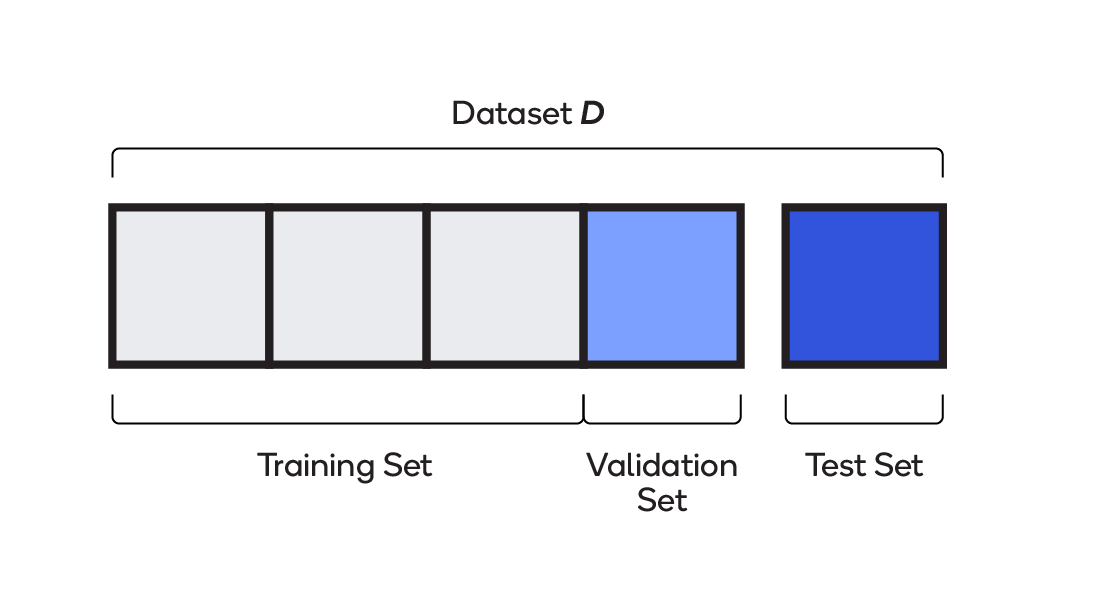
\includegraphics[width=\textwidth]{imatges/preliminaries/train-test-validation-sets.png}
  \end{adjustbox}
  \caption[Holdout Set Scheme]{\textit{Holdout Set Scheme. Illustration by Qualcomm}}
  {\label{fig:holdout-test-scheme}}
\end{figure}

The Holdout set scheme involves dividing the data into two sets: one for
training and another for testing. Additionally, a validation set is created
from the training set to assess how well the model performs on unseen data
during training. \\

During the training phase, the test set remains completely separate and is not
used in any way to configure the hyper-parameters. This ensures that the
model's performance on the validation set is not artificially inflated by
adjusting hyper-parameters to achieve an exceptionally good outcome. \\

The data from the ISIC Archive was divided using the following percentages: 80%
for training, 10\% for validation, and 10\% for testing.

\section{Test-Time Augmentation}

Test-time augmentation (TTA) is used during the testing or inference phase of a
machine learning model. TTA generates multiple augmented versions of test
samples to obtain diverse predictions. By obtaining predictions from these
augmented samples and combining them, TTA mimics the behavior of an ensemble of
models.

\begin{figure}[H]
  \centering
  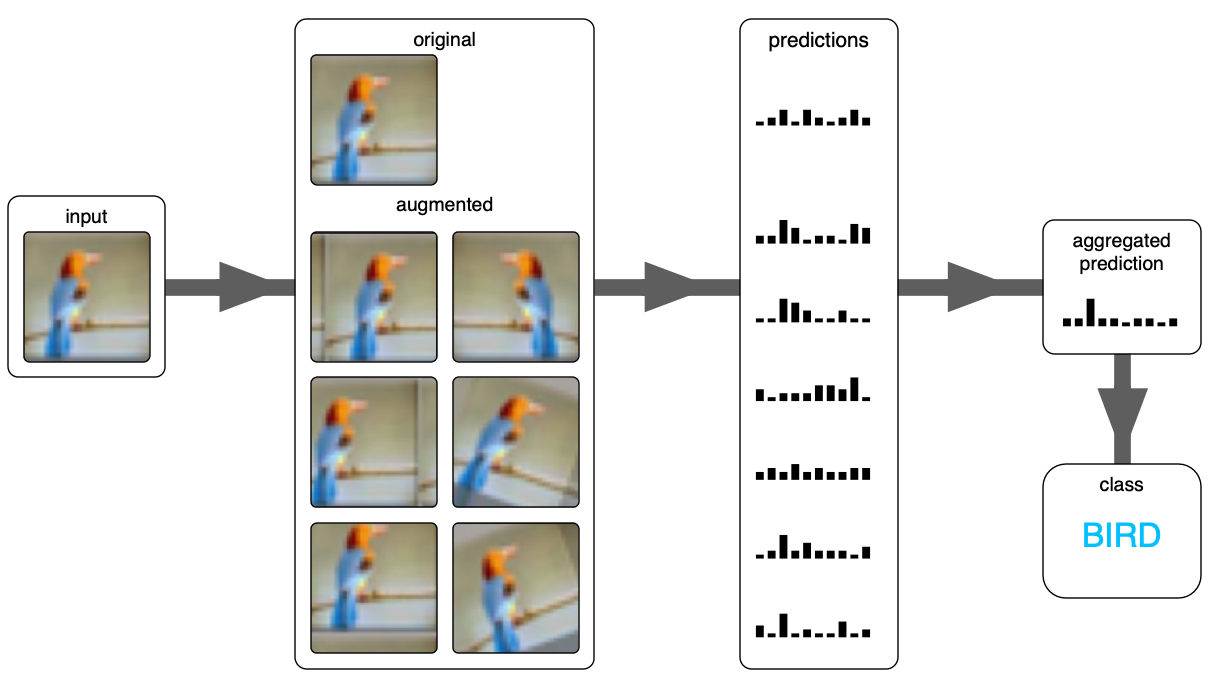
\includegraphics[width=0.8\textwidth]{imatges/preliminaries/tta.png}
  \caption[Test-Time Augmentation]{\textit{Test-Time Augmentation. Illustration by stepup.ai}}
  {\label{fig:tta}}
\end{figure}

\newpage

\section{ResNet}

ResNet, short for "Residual Network," is a deep convolutional neural network
(CNN) architecture that was introduced in 2015 by researchers from Microsoft
Research \cite{ResNetPaper}. It revolutionized the field of deep learning by
addressing the challenge of training very deep neural networks. \\

The main problem encountered when training deep neural networks is the
degradation problem, where the accuracy of the model saturates and then starts
to decline rapidly as the network depth increases. This degradation occurs due
to the difficulty of optimizing the network's parameters and the vanishing
gradient problem, where gradients become extremely small during
backpropagation, making it difficult for the network to learn effectively.
\\

ResNet tackled this problem by introducing the concept of residual learning.
The key idea is to use "skip connections" or "identity mappings" that allow the
network to learn residual functions. Instead of trying to learn the underlying
mapping directly, ResNet models learn the residual between the desired mapping
and the input. \\

By introducing these skip connections, ResNet models can effectively "skip" one
or more layers during training, allowing information to flow more easily
through the network. This mitigates the degradation problem and enables the
training of extremely deep networks (e.g., hundreds of layers) without
suffering from diminishing accuracy. \\

In ResNet, each layer of the network contains a residual block. A residual
block consists of multiple convolutional layers followed by batch normalization
and activation functions. The input to a residual block is added to its output
through a skip connection, which directly connects the input to the output.
This allows the network to learn the residual information, or the difference
between the input and the desired output, making it easier for the network to
learn the underlying mapping.  \\

There are various architectural variants or "flavors" of ResNet, including
ResNet-152,  ResNet-101,  ResNet-50,  ResNet-34, and  ResNet-18. The
number following the name of each ResNet variant indicates the number of inner
layers present in the architecture.

\newpage

As evident from Figure \ref{fig:resnet}, it can be observed that
ResNet architectures with a greater number of layers tend to exhibit higher
accuracy. However, it is important to note that this improvement in accuracy
comes at the expense of having a significantly larger number of parameters to
train.


\begin{figure}[H]
  \begin{adjustbox}{width=\textwidth, trim={0pt 0pt 1cm 0pt}, clip}
    \centering
    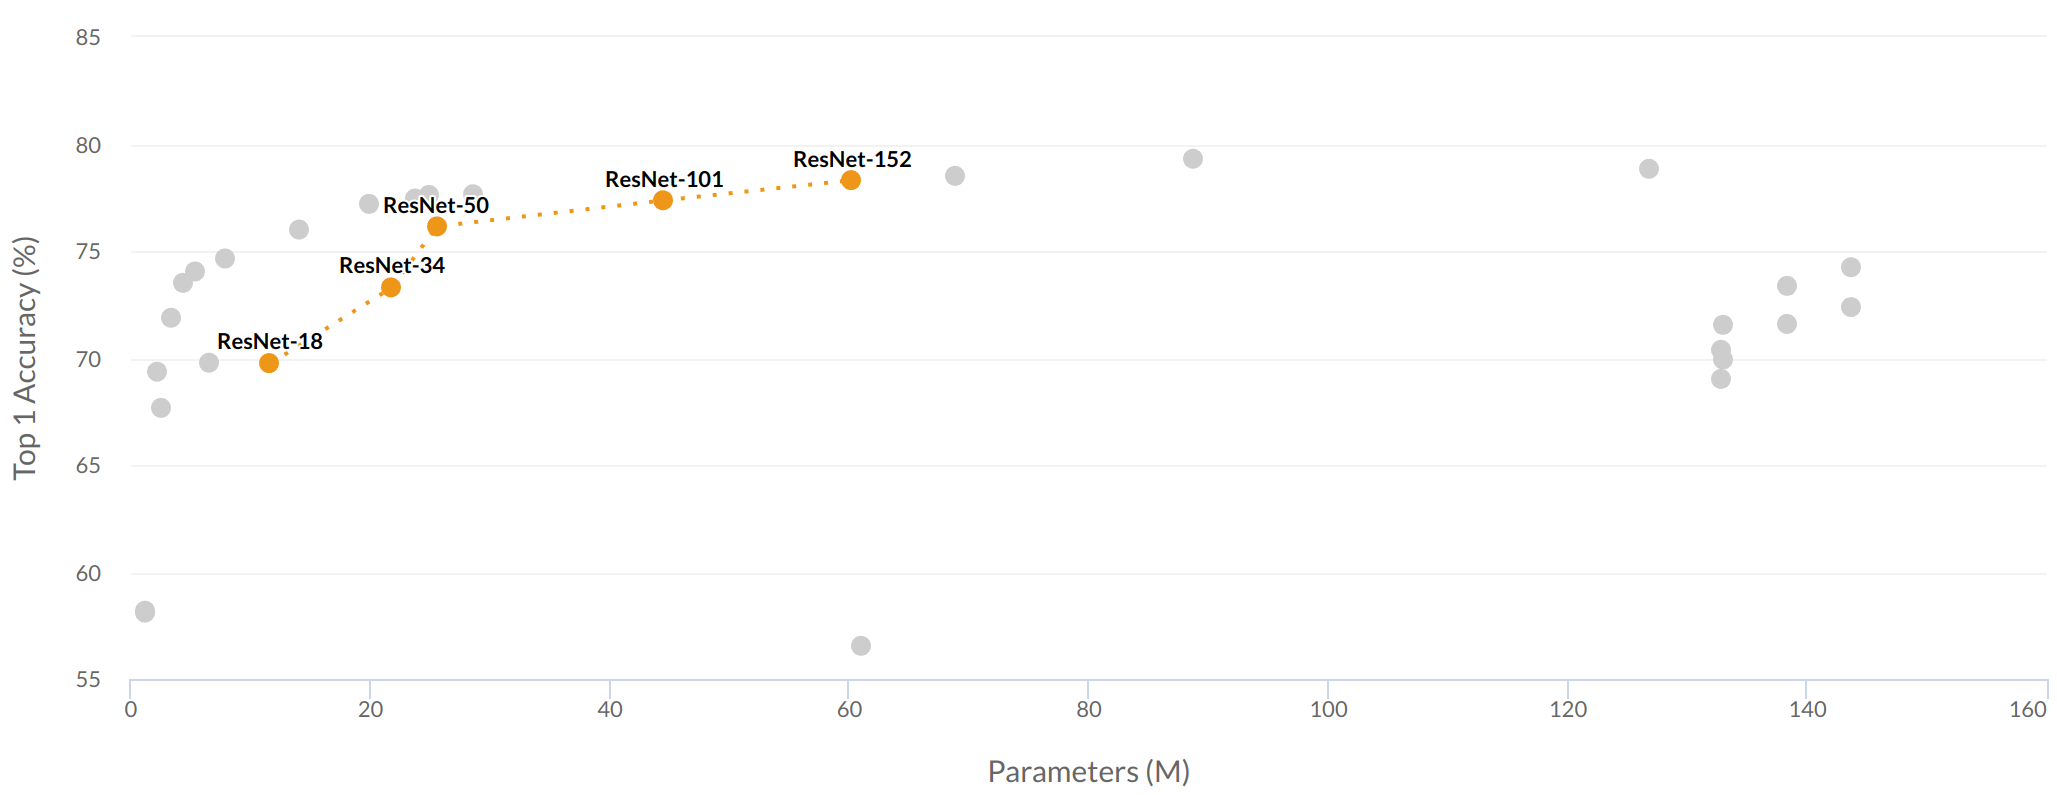
\includegraphics[width=\textwidth]{imatges/preliminaries/ResNetImageNet.png}
  \end{adjustbox}
  \caption[ResNet "flavors" Results on ImageNet]{\textit{ResNet "flavors" Results on ImageNet. Illustration by paperswithcode}}
  {\label{fig:resnet}}
\end{figure}

To accurately assess the performance of each ResNet architecture, refer to
Table \ref{table:resnet}, which provides the accuracy achieved on the ImageNet
dataset along with the corresponding number of trainable parameters in
millions.

\begin{table}[H]
  \centering
  \begin{tabular}{lcc}
    \toprule
    \textbf{Model} & \textbf{Accuracy} & \textbf{Parameters} \\
    \midrule
    ResNet-152 & 78.31\% & 60.2M \\
    ResNet-101 & 77.37\% & 44.5M \\
    ResNet-50 & 76.15\% & 25.6M \\
    ResNet-34 & 73.30\% & 21.8M \\
    ResNet-18 & 69.76\% & 11.7M \\
    \bottomrule
  \end{tabular}
  \caption[Accuracy achieved on ImageNet and trainable parameters of each resNet.]
  {\textit{Accuracy achieved on ImageNet and trainable parameters of each resNet.
  Each image in the ImageNet dataset is associated with 1 of 1,000 classes. Table by paperswithcode}}
  {\label{table:resnet}}
\end{table}

\section{Micro-services Architecture}

A micro-services architecture is a software design approach that structures an
application as a collection of small, independent services, each running in its
own process and communicating with each other through lightweight mechanisms.
This architecture promotes scalability, modularity and flexibility. \\

As a result of this thesis we built two services: an API and a UI. These services
are built using different frameworks and programming languages.

\section{Inference API}

The inference API service focuses on handling the back-end logic and data
processing. It exposes a well-defined API that allows user to interact with the
trained models. \\

The end-points that the present thesis API service support are explained in
Section \ref{cap:result}.

\section{Containerization}

Containerization is a technology that allows applications and their
dependencies to be packaged into isolated, lightweight containers. These
containers provide an encapsulated runtime environment, ensuring that the
application runs consistently across different systems. \\

Containers are created from container images, which are self-contained packages
containing the application's code, dependencies, libraries, and configurations.
Images serve as the blueprint for creating containers. They can be shared,
versioned, and easily deployed on various platforms. \\

Frameworks such as Docker and Podman, provide tools and services to build,
manage, and run containers. These frameworks utilize underlying virtualization
technologies to create and manage isolated environments. These environments,
called containers, offer resource isolation and ensure that applications run
consistently across different computing environments. As a result, services
running in containers are easy to maintain, portable and fast to start-up.

\section{Platform Deployment}

To distribute the containerized API and UI services easily to professionals,
there are several solutions available. In this thesis, we propose the creation
of a shell script that performs the following steps:

\begin{itemize}
  \item Creates a directory in the system's home directory to download the source code and artifacts.
  \item Clones the source code repository from GitHub.
  \item Moves the encapsulated Python packages into the API source code.
  \item Builds the API image.
  \item Builds the UI image.
  \item Clones the artifacts from GitLab.
  \item Activates the services using a Docker Compose file, which starts the containers with their configurations based on the previously built images.
\end{itemize}

By following this approach, professionals can easily distribute the
containerized services by running the provided shell script.
